\chapter{Solution Design: Improved Kepler Visualisation Tool}\label{C:sd}

This section discusses the design of the deliverable visualisation that was created as part of this project. It details decisions made during the project such as choosing a viable framework, the choice of extending a previous system,   platform choice, and designs of the actual system.   

\section{Technology choice}
Many technologies were looked into,experimented with, and the positives and negatives of each weighed up before a decision was made about which would be the choice for the visualisation. It came down to 3 potential technologies that would be suitable for the project, the next 3 subsections outline these in detail.

\subsubsection{D3 (Data Driven Documents)}
D3 is a JavaScript library that allows the displaying of data in dynamic graphics. Embedded
within an HTML web page, the JavaScript D3.js library uses pre-built JavaScript functions to
select elements, create Scalable Vector Graphic (SVG)[17] objects, style them, and add transitions,
dynamic effects and tooltips. Large datasets can be easily bound to SVG objects using
simple D3 functions to generate rich charts and diagrams. D3 was created because of the
need for a balance of expressiveness, efficiency, and accessibility that previous visualization
toolkits did not allow [4].

D3 allows the binding of input data to arbitrary input elements. This means that the exoplanet
dataset can easily be bound to SVG elements for creating visualizations. D3 adopts
the W3C Selectors API to identify document elements queried. This results in a rich but
concise selection method of elements in a visualisation.

D3 allows debugging thanks to Google chrome and other modern browsers development
tools. A downside to D3 is that it does not allow 3D diagrams, although it does allow
pseudo 3D by using the painter’s algorithm and 3D textures.

\subsubsection{Prefuse}
Prefuse is a set of software tools for creating rich interactive data visualizations [13]. The
Prefuse toolkit provides a visualization framework for Java. It supports a set of features
for visualizing and interacting with data. It provides optimized data structures for tables,
graphs, and trees. It can be used to build standalone applications, visual components embedded
in larger applications, and web applets. Prefuse to greatly simplifies the process
of representing and efficiently handling data, mapping data to visual representations (e.g.,
through spatial position, size, shape, color, etc), and interacting with the data.
To use Prefuse a basic familiarity with the Java is required, including setting up and building
Java projects. A knowledge of Swing or another similar user interface toolkit is also
useful for understanding some of the concepts behind Prefuse and for integrating Prefuse
visualizations into larger applications. Experience with database systems is also helpful. 
However the complexity of Prefuse means that the learning curve will be out of scope for
this project.

\subsubsection{Processing}
Processing is an open source programming language and development environment that was initially created to serve as a software
sketchbook and to teach the fundamentals of computer programming with a visual context.
Using processing would mean that the visualization could be built with Java while still using
a successful visualisation framework. The most complete existing visualization using
the same exoplanet dataset (Kepler Visualization Tool) is built using Processing.
Using this solution would involve learning the Processing language, however Processing
is a library built in Java so the syntax is the same. This means the learning curve should be shallow.
Using processing means that 3D elements could be included, this wouldnt be
possible with D3.

\subsubsection{Decision of technology}
The final decsion of techology was to use Processing, this is because it had many positive aspects that the others did not and minimal nigatives as the below table illistrates.
\clearpage
\begin{figure}[h!]
  \centering
      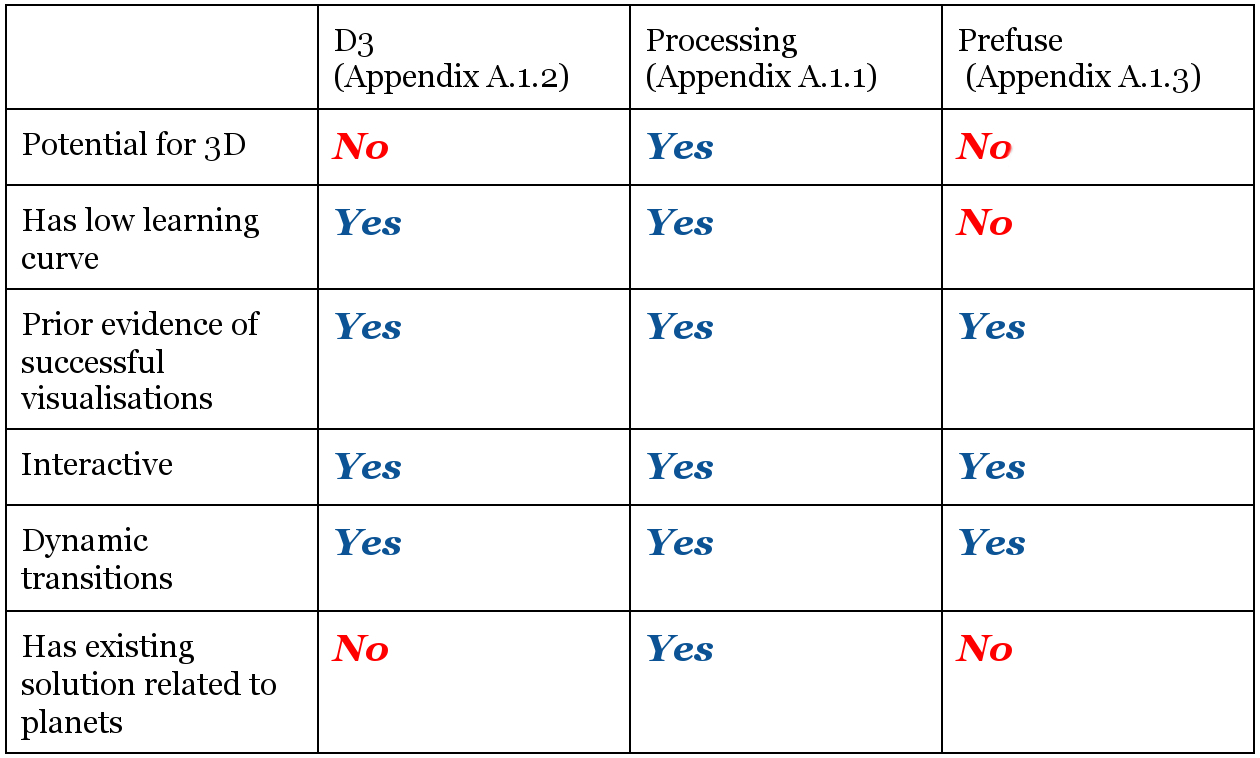
\includegraphics[width=0.8\textwidth]{images/table_technologies.jpg}
  \caption{Table of technology choices}
\end{figure}

As this project was created using Processing, it allowed me to extend the previous visualisation using the same data set, The Kepler Visualisation Tool \cite{kepler_github, kepler_article}. As the time was short for this project builing upon a previous solution increased the amount of progress that could be made in the time afforded.
\\\\
Taking this approach meant that the languages being used would be Java using processing libraries. 

As this is such a large project involving many different iterations, version control was important for maintaining records and backups of important changes which was stored on remote servers to ensure against file loss in system failures.

\section{System design and structure}
BASIC Class structure

Data structure

UML CLass Diagram


\section{Visualisation Design}
The visualisation was designed to emphasis small multiples and filtering of the Exoplanets to display the information more clearly to users. 
\\\\
Instead of the visualisation only answering the 5 key questions as proposed in the proposal, the aim will now be displaying as much of the information in the dataset as possible without detracting from the effectiveness of the visualisation whilst still answering the questions. 
\\\\
This is because the 5 questions did not fully utilize the information in the dataset. 
\\\\
However I will need to ensure the effectiveness of the visualisation does not become diminished by trying to convey to much information which would lead to cluttering and overlapping in the visualisation, as well as information overload for users. There will also be larger emphasis placed on making the existing system more usable by improving the interaction methods for users. The following list outlines the new requirements for the visualisation being developed. This will be done by 
providing GUI elements for each form of interaction with the system, as well as ensuring all interaction methods are intuitive for users. 
\subsubsection{Spacial arrangement}
As the majority of the interaction and movement of visualisation elements occurs in the center of the window it caused a aspect ratio that was not suitable . It was BETTER~ to use 2 vertical columns to view and control the visualisation as it had a higher aspect ratio which allowed more of the content to be seen on the screen at once thanks to the fact that the majority of computer screens have a wide ratio.

\begin{figure}[h!]
  \centering
      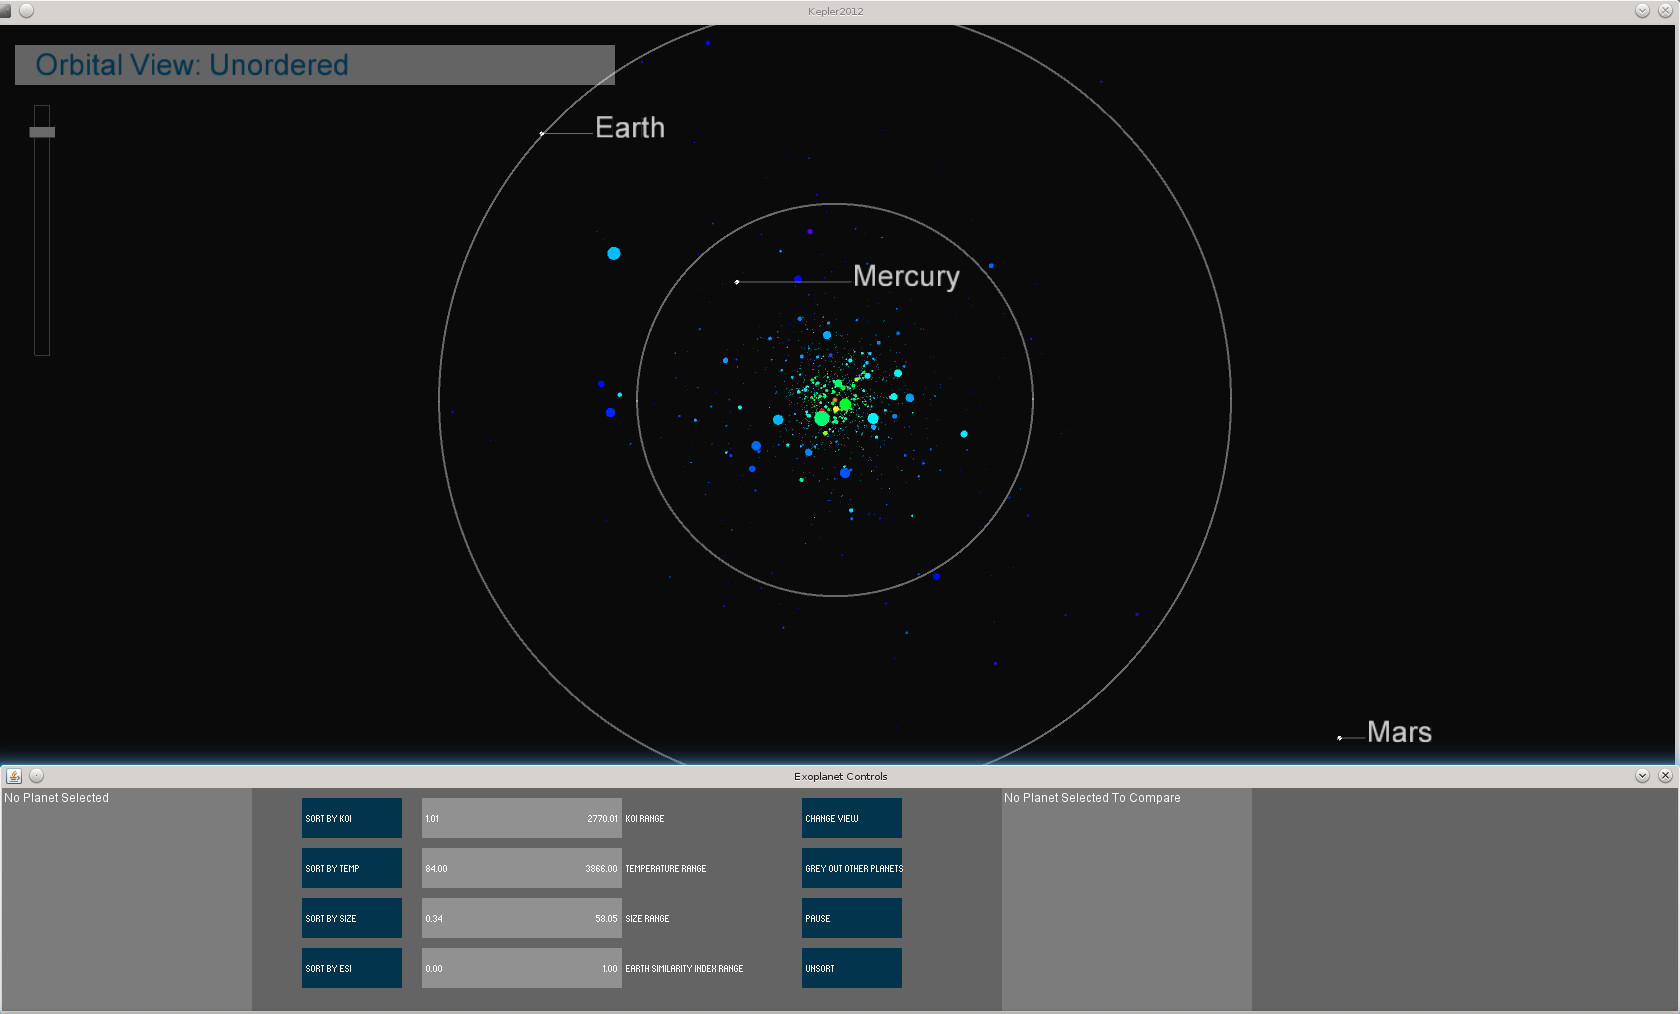
\includegraphics[width=0.8\textwidth]{images/layout_horizontal.jpg}
  \caption{Original Horizontal Layout}  
        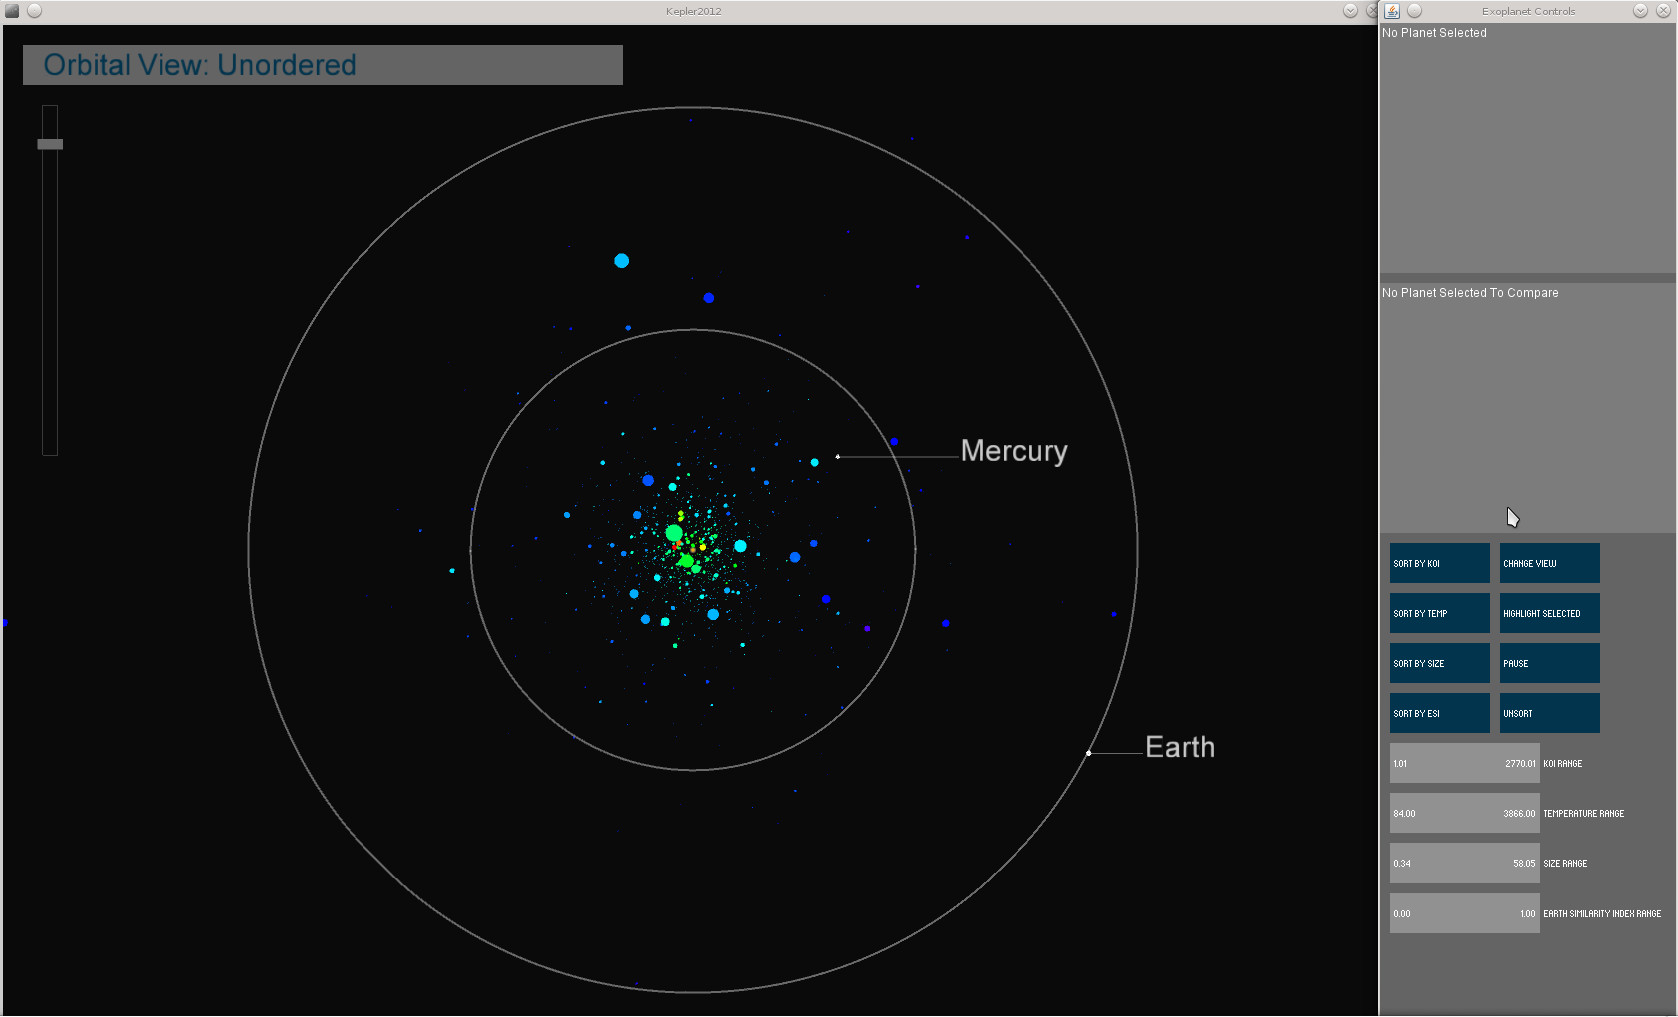
\includegraphics[width=0.8\textwidth]{images/layout_vertical.jpg}
  \caption{Improved Vertical Layout}
\end{figure}

\subsubsection{Navigation Window(BETTER TITLE~)}
Description of navigation window

Description of each button

Description of each slider

Description of text boxes

Due to the need for increased user interaction with the visualisation a window is required to house the buttons, range selectors, and text areas. These elements are needed as the different methods that users can use to interact with the visualistaion need to be visually apparent to ensure that the system can be easily used without prior experience. A way to do this is to provide clearly labelled interactive elements and tooltips explaining what they do.((REFERENCE))~. These tooltips are widely used as a method of informing a user about the purpose of an item by hovering over it. This removes the need to click on a button to discover its effect.

\subsubsection{Visualisation Layout for Kinect sensor}
As the Kinect sensor no longer requires the use of a mouse the visualisation design needs to be modified to accomodate the use of gestures. For this project this meant incorporating new cursers to indicate the state of the visualisation. There are 7 states that the curser needs to be able to be in to inform the user of what action they are performing. These states are

\begin{enumerate}
 \item default curser, hand is at rest
 \item panning up, hand is raised
 \item panning down, hand is lowered
 \item panning left, hand is to the left
 \item panning right, hand is to the right
 \item zooming in, hand is pressed forward
 \item zooming out, hand is pulled backwards
\end{enumerate}

Having a range of icons that clearly display these states is vital for keeping the user informed of what they are doing. The icons designed for this purpose are in the following figure

\begin{figure}[h!]
  \centering
  ~
      %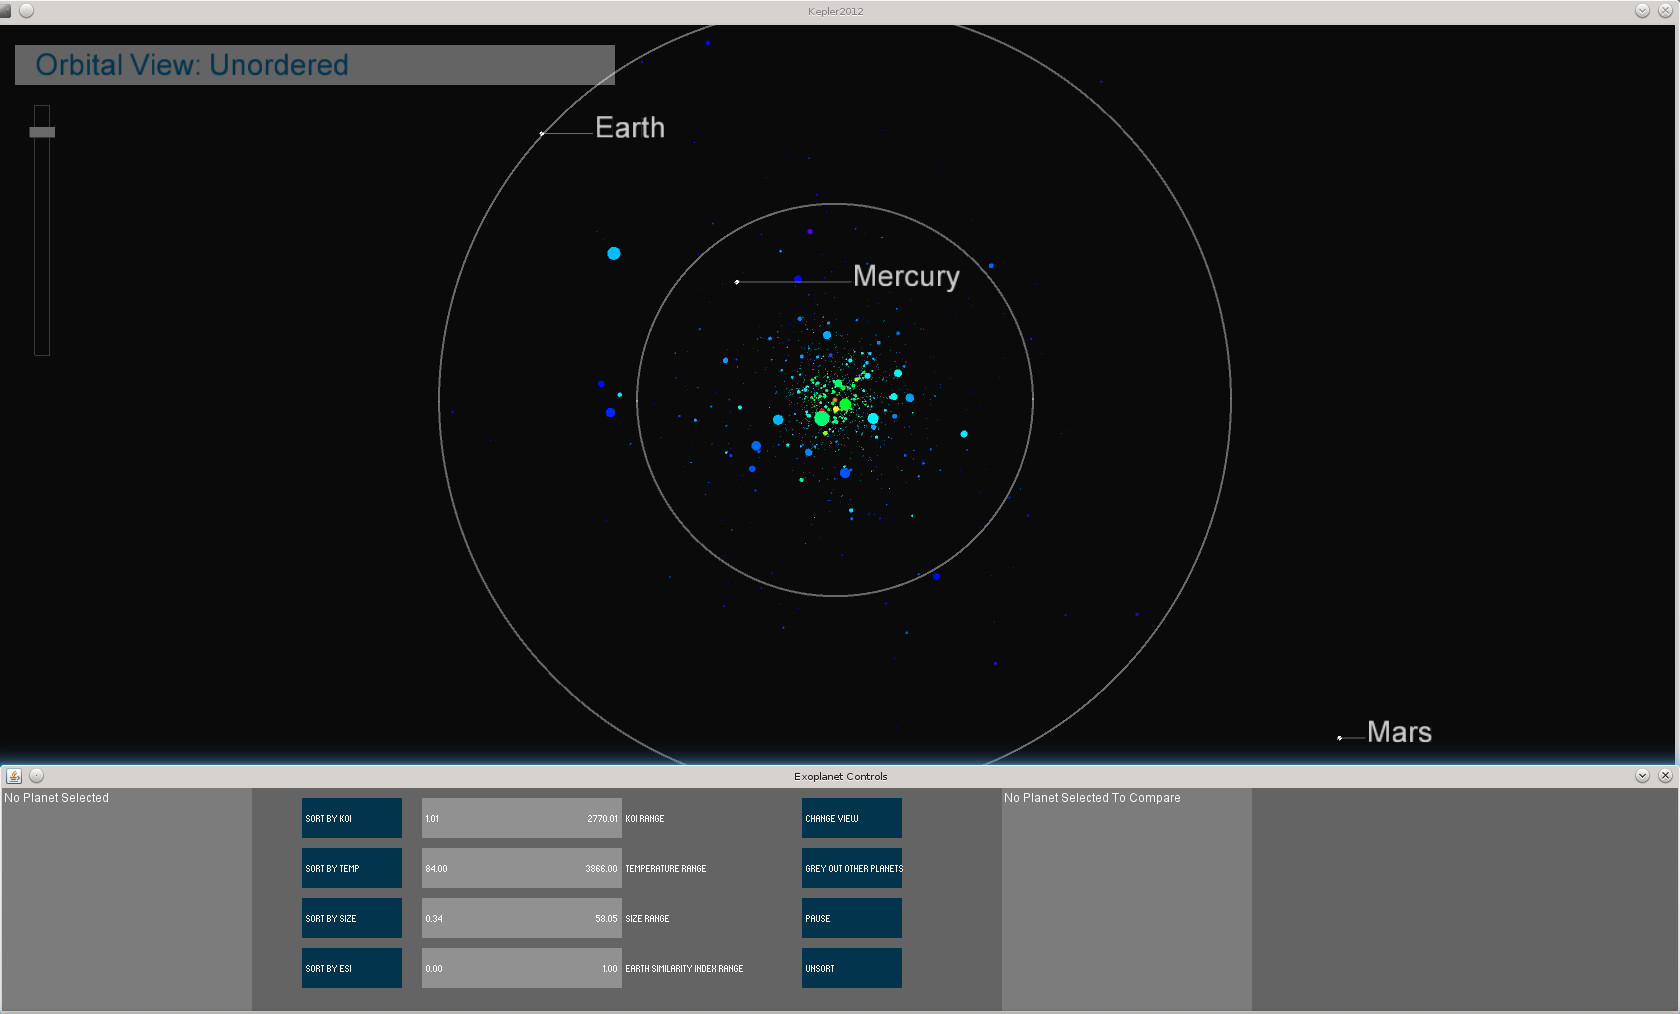
\includegraphics[width=0.8\textwidth]{images/layout_horizontal.jpg}
  \caption{Cursers for Kinect sensor}  
\end{figure}

In addition to this, the screen needs to display the user in relation to the screen, an effective way to do this is to display a washed out representation of themselves in the background of the visualisation. 